%--------------------
% Document type
% -------------------
\documentclass[11pt,a4paper]{article}

%-----------------------
% Input a file which contains all the setup 
%-----------------------
\usepackage[utf8x]{inputenc}
\usepackage[T1]{fontenc}
%\usepackage{mathptmx} % Use Times Font
\usepackage{cmbright} % Use Sans-Serif Font
\usepackage[pdftex]{graphicx} % Required for including pictures
\usepackage[pdftex,linkcolor=black,pdfborder={0 0 0}]{hyperref} % Format links for pdf
\usepackage{calc} % To reset the counter in the document after title page
\usepackage{enumitem} % Includes lists

\usepackage[a4paper, lmargin=0.1666\paperwidth, rmargin=0.1666\paperwidth, tmargin=0.1111\paperheight, bmargin=0.1111\paperheight]{geometry} %margins
%\usepackage{parskip}

\usepackage[all]{nowidow} % Tries to remove widows
\usepackage[protrusion=true,expansion=true]{microtype} % Improves typography, load after fontpackage is selected

\usepackage{amsmath}     % For mathematical equations

\usepackage{booktabs}    % For table formatting

\usepackage{algorithm}
\usepackage{algpseudocode}

\usepackage{caption}    % For Figures
\usepackage{subcaption}
\usepackage{xcolor}


%-----------------------
% Set pdf information and add title, fill in the fields
%-----------------------
\hypersetup{ 	
pdfsubject = {},
pdftitle = {Kinematics and Trajectory Workshop},
pdfauthor = {}
}

%-----------------------
% Begin document
%-----------------------
\begin{document}

%-----------------------
% Title, author and date
%-----------------------

\title{\bfseries\huge Kinematics and Trajectory Workshop}
\author{Michael Ziegltrum}
\date{\today}
\maketitle

\section{Introduction}

In this series of labs we will explore fundamentals of robotics in the contex of a robotic arm. This will involve implementing and tuning algorithms first in simulation then on a real robot to figure out where the arm is and control it to achieve a writing task. 

There are some prerequisites needed to do these lab activities. Please fulfill these prior to the lab.

\begin{enumerate}
    \item{A working Ubuntu 22.04 installation, for Windows and Mac users via a virtual machine provider like VirtualBox \url{https://www.virtualbox.org/}.}
    \item{Docker engine installed inside of the Ubuntu installation \url{https://docs.docker.com/engine/install/ubuntu/}. Please test by running the command `sudo docker run hello-world` and ensure no error output.}
    \item{About 50Gb free space on the computer.}
    \item{Basic familiarity with ROS (ROS2 Humble) will help, doing the CLI tools tutorials and the client library tutorials up to "writing a simple publisher and subscriber" is recommended \url{https://docs.ros.org/en/humble/Tutorials/Beginner-CLI-Tools.html}}
\end{enumerate}

The LaTex source code for this file is included in the code repository. It is intended for students to use this template to respond to the questions (in red) with their answers (in blue).

\section{Running the Simulation and Introspection}

In this section we will run the simulation and understand how the pieces of the software stack are used together.

Please build the docker file and run the simulation by following the instructions in the README.md in the code repository \url{https://github.com/MZandtheRaspberryPi/kinematics_workshop}. You should see a window like in figure \ref{fig:pybullet} come up, which is the Graphical User Interface (GUI) of Pybullet \cite{coumans2016pybullet}, a simulator we use for the workshop. To rotate the camera hold control and left click and drag the mouse. To translate the camera hold control and hold the mouse wheel and drag the mouse. To enable/disable wireframe mode press "w" and to visualize joints when in wireframe mode press "j".

\begin{figure}[h]
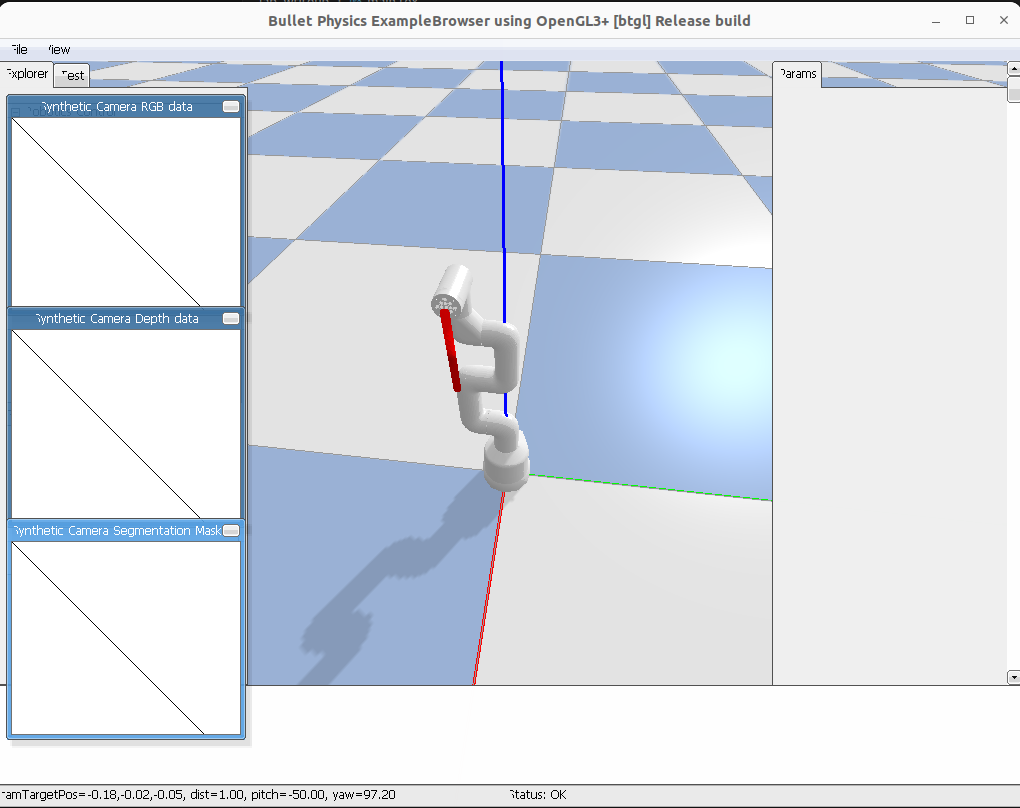
\includegraphics[width=8cm]{figures/pybullet.png}
\centering
\caption{The pybullet simulator Graphical User Interface (GUI) that we use for the workshop.}
\label{fig:pybullet}
\end{figure}

ROS2 is a middleware based on a publish/subscribe mechanism where various processes (nodes) send and receive information (messages) via various paths (topics). By using introspection tools detailed in the Beginner CLI tools tutorials answer the following questions:

\subsection{Question 1--System Overview}

Run the simulator in addition to the controller. 

\textcolor{red}{How many nodes are running in the system and what are their names? }

\textcolor{blue}{Answer: }

\textcolor{red}{Which topics do they each publish to, and what information is included in the messages they pass back and forth? Give an example of each message in text format included in the write-up. Hint: in addition to the other tools overviewed in the CLI tutorials, the rqt\_graph tool may be espically helpful to understand the system more broadly.}

\textcolor{blue}{Answer: }

\subsection{Question 2--Simulator Node}

The node that is responsible for running the pybullet simulation is in the ros\_sim package, and the source code is in the ros\_sim/pybullet\_ex.py file. There are multiple timesteps used in the triggering of the simulation step including the timestep for pybullet, the timestep for the wrapper around pybullet and the ROS2 callback timer. 

\textcolor{red}{What function is responsible for stepping the simulation and propogating dynamics, and what timestep does it use for the simulation?}

\textcolor{blue}{Answer: }


\textcolor{red}{What are the tradeoffs involved in changing the timestep used for the Pybullet simulation to something very large (a second), compared to something very small (a thousandth of a second)?}

\textcolor{blue}{Answer: }

One critical choice is in the modelling of the robot's motion. Using commands in the README, bring up the pybullet simulator and publish a goal for the arm. What does the motion look like? The ros\_sim package uses PositionControl mode where pybullet models a Proportional Derivative controller at each joint that looks at position goals and velocity, and calculates force to apply to the joint. In the reset function is an example of resetting a joint's state without using a PD controller. Change the step function to use the joint reset for each joint instead of the PD controller (the pybullet quick start guide is helpful for function documentation \url{https://docs.google.com/document/d/10sXEhzFRSnvFcl3XxNGhnD4N2SedqwdAvK3dsihxVUA/edit?tab=t.0#heading=h.2ye70wns7io3}), and run the pybullet simulation and publish a goal for the arm using commands in the README.

\textcolor{red}{ What behavior do you notice? Which method (PD controller vs Resetting Joint State) would track a given trajectory more closely? Which method would match the real robot better?}

\textcolor{blue}{Answer: }

Revert your changes to the step function.

\subsection{Question 3--Controller Node}

The node that is responsible for commanding the arm is in the ros\_arm\_controller package, and the source code is in the ros\_arm\_controller/robo\_controller.py file. In the README commands to run the node a simulation time parameter is used.

\textcolor{red}{ What is the impact of the simulation\_time parameter and what would happen if the controller was running in real time while the simulator was unchanged? Hint: look at ros2 documentation on simulation time.}

\textcolor{blue}{Answer: }

\clearpage

\section{Forward Kinematics}

One fundamental problem in robotics is going from the joint angles of the robot to the position of some key frame on the robot. This section will explore this problem.

\subsection{Question 1--DH Params}

The robot model is in a Unified Robot Description Format (URDF) file \url{https://docs.ros.org/en/humble/Tutorials/Intermediate/URDF/URDF-Main.html} located in the ros\_sim package under resource/robots/mycobot\_280\_pi/mycobot\_280\_pi\_mod.urdf. In this lab we will to try draw patterns using a marker attached to the robot.

\textcolor{red}{ What is the name of the link at the tip of the pen that we wish to control? }

\textcolor{blue}{Answer: }

ROS has it's own forward kinematic algorithms, but the Denavit-Hartenberg parameters are still a useful construct \cite{denavit1955kinematic} to model the forward kinematics of a robot arm. Figure \ref{fig:dh_diagram} shows a kinematic diagram following the DH conventions and figure \ref{fig:dh_table} shows the parameters, provided by the manufacturer \cite{er_dh_param}. However, there are two gaps. One is that we will attach a base to the robot that provides a space to clamp the robot onto the table. The base is 0.029 meters high and will result in the entire robot moving upward in z. The second gap is that we mount the pen to the robot arm using a piece designed and fabricated by Alex Charitonidis shown in figure \ref{fig:pen_mount}. The distance from the middle of the robot's wrist to the tip of the pen, along the axis normal to the z-axis of the wrist and the pen, is 40mm. The distance from the middle of the robot's wrist to the tip of the pen, along the wrist's z-axis, is around 35mm though this can be modified by sliding the pen back or forward and should be verified. Another crucial information is where is the pen tip when the wrist joint is set to 0 degrees. Figure \ref{fig:pen_mount} shows this configuration. If a circle were drawn centering at the robot's wrist, where the tip of the pen aligns with a point on the circle's circumference (with a radius of 40mm from the center), and the point is in the first quadrant of the unit circle, the angle is 45 degrees between the hypotenuse drawn to the pen tip and the x-axis. However, the DH parameters may use a different convention for the prior frame and put X somewhere else. 


\begin{figure}[h]
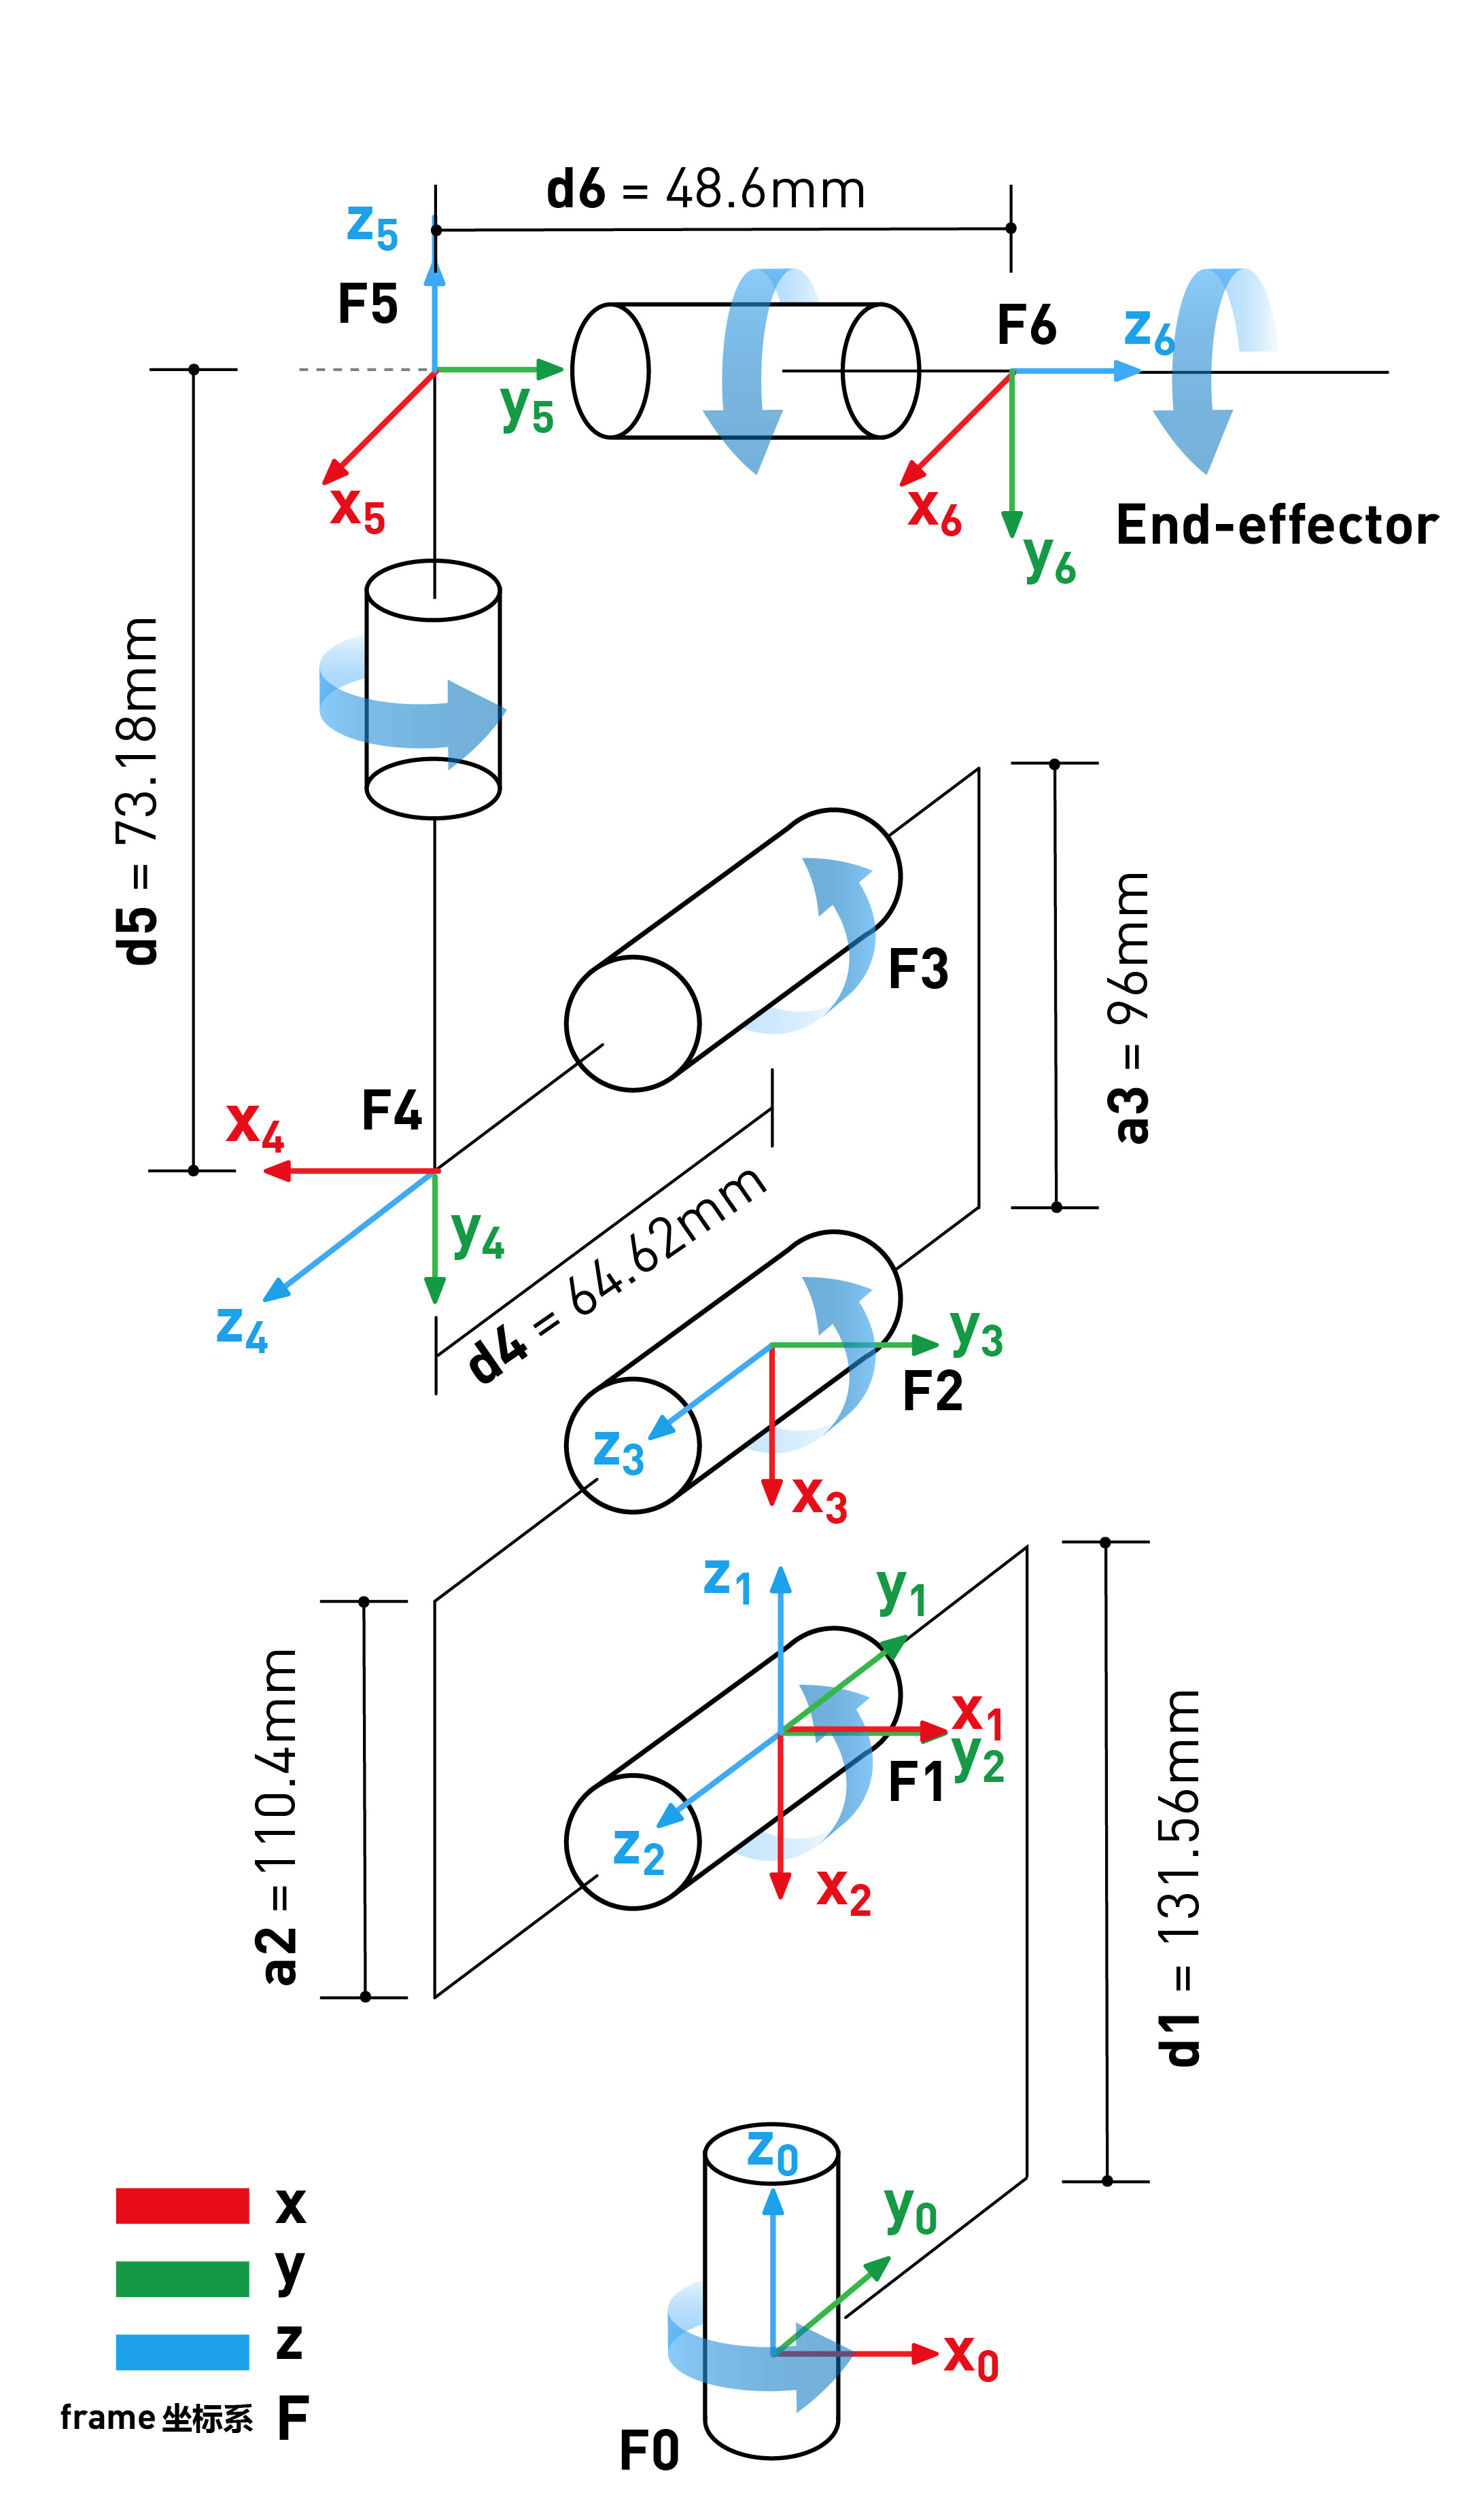
\includegraphics[width=8cm]{figures/dh_params_manufacturer.jpg}
\centering
\caption{Kinematic diagram of the Mycobot 280 Raspberry Pi, provided by the manufacturer.}
\label{fig:dh_diagram}
\end{figure}

\begin{figure}[h]
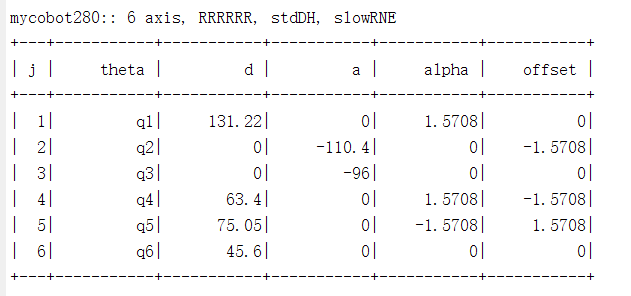
\includegraphics[width=8cm]{figures/dh_params_table.png}
\centering
\caption{Denavit-Hartenberg parameters of the Mycobot 280 Raspberry Pi, provided by the manufacturer.}
\label{fig:dh_table}
\end{figure}

\begin{figure}[h]
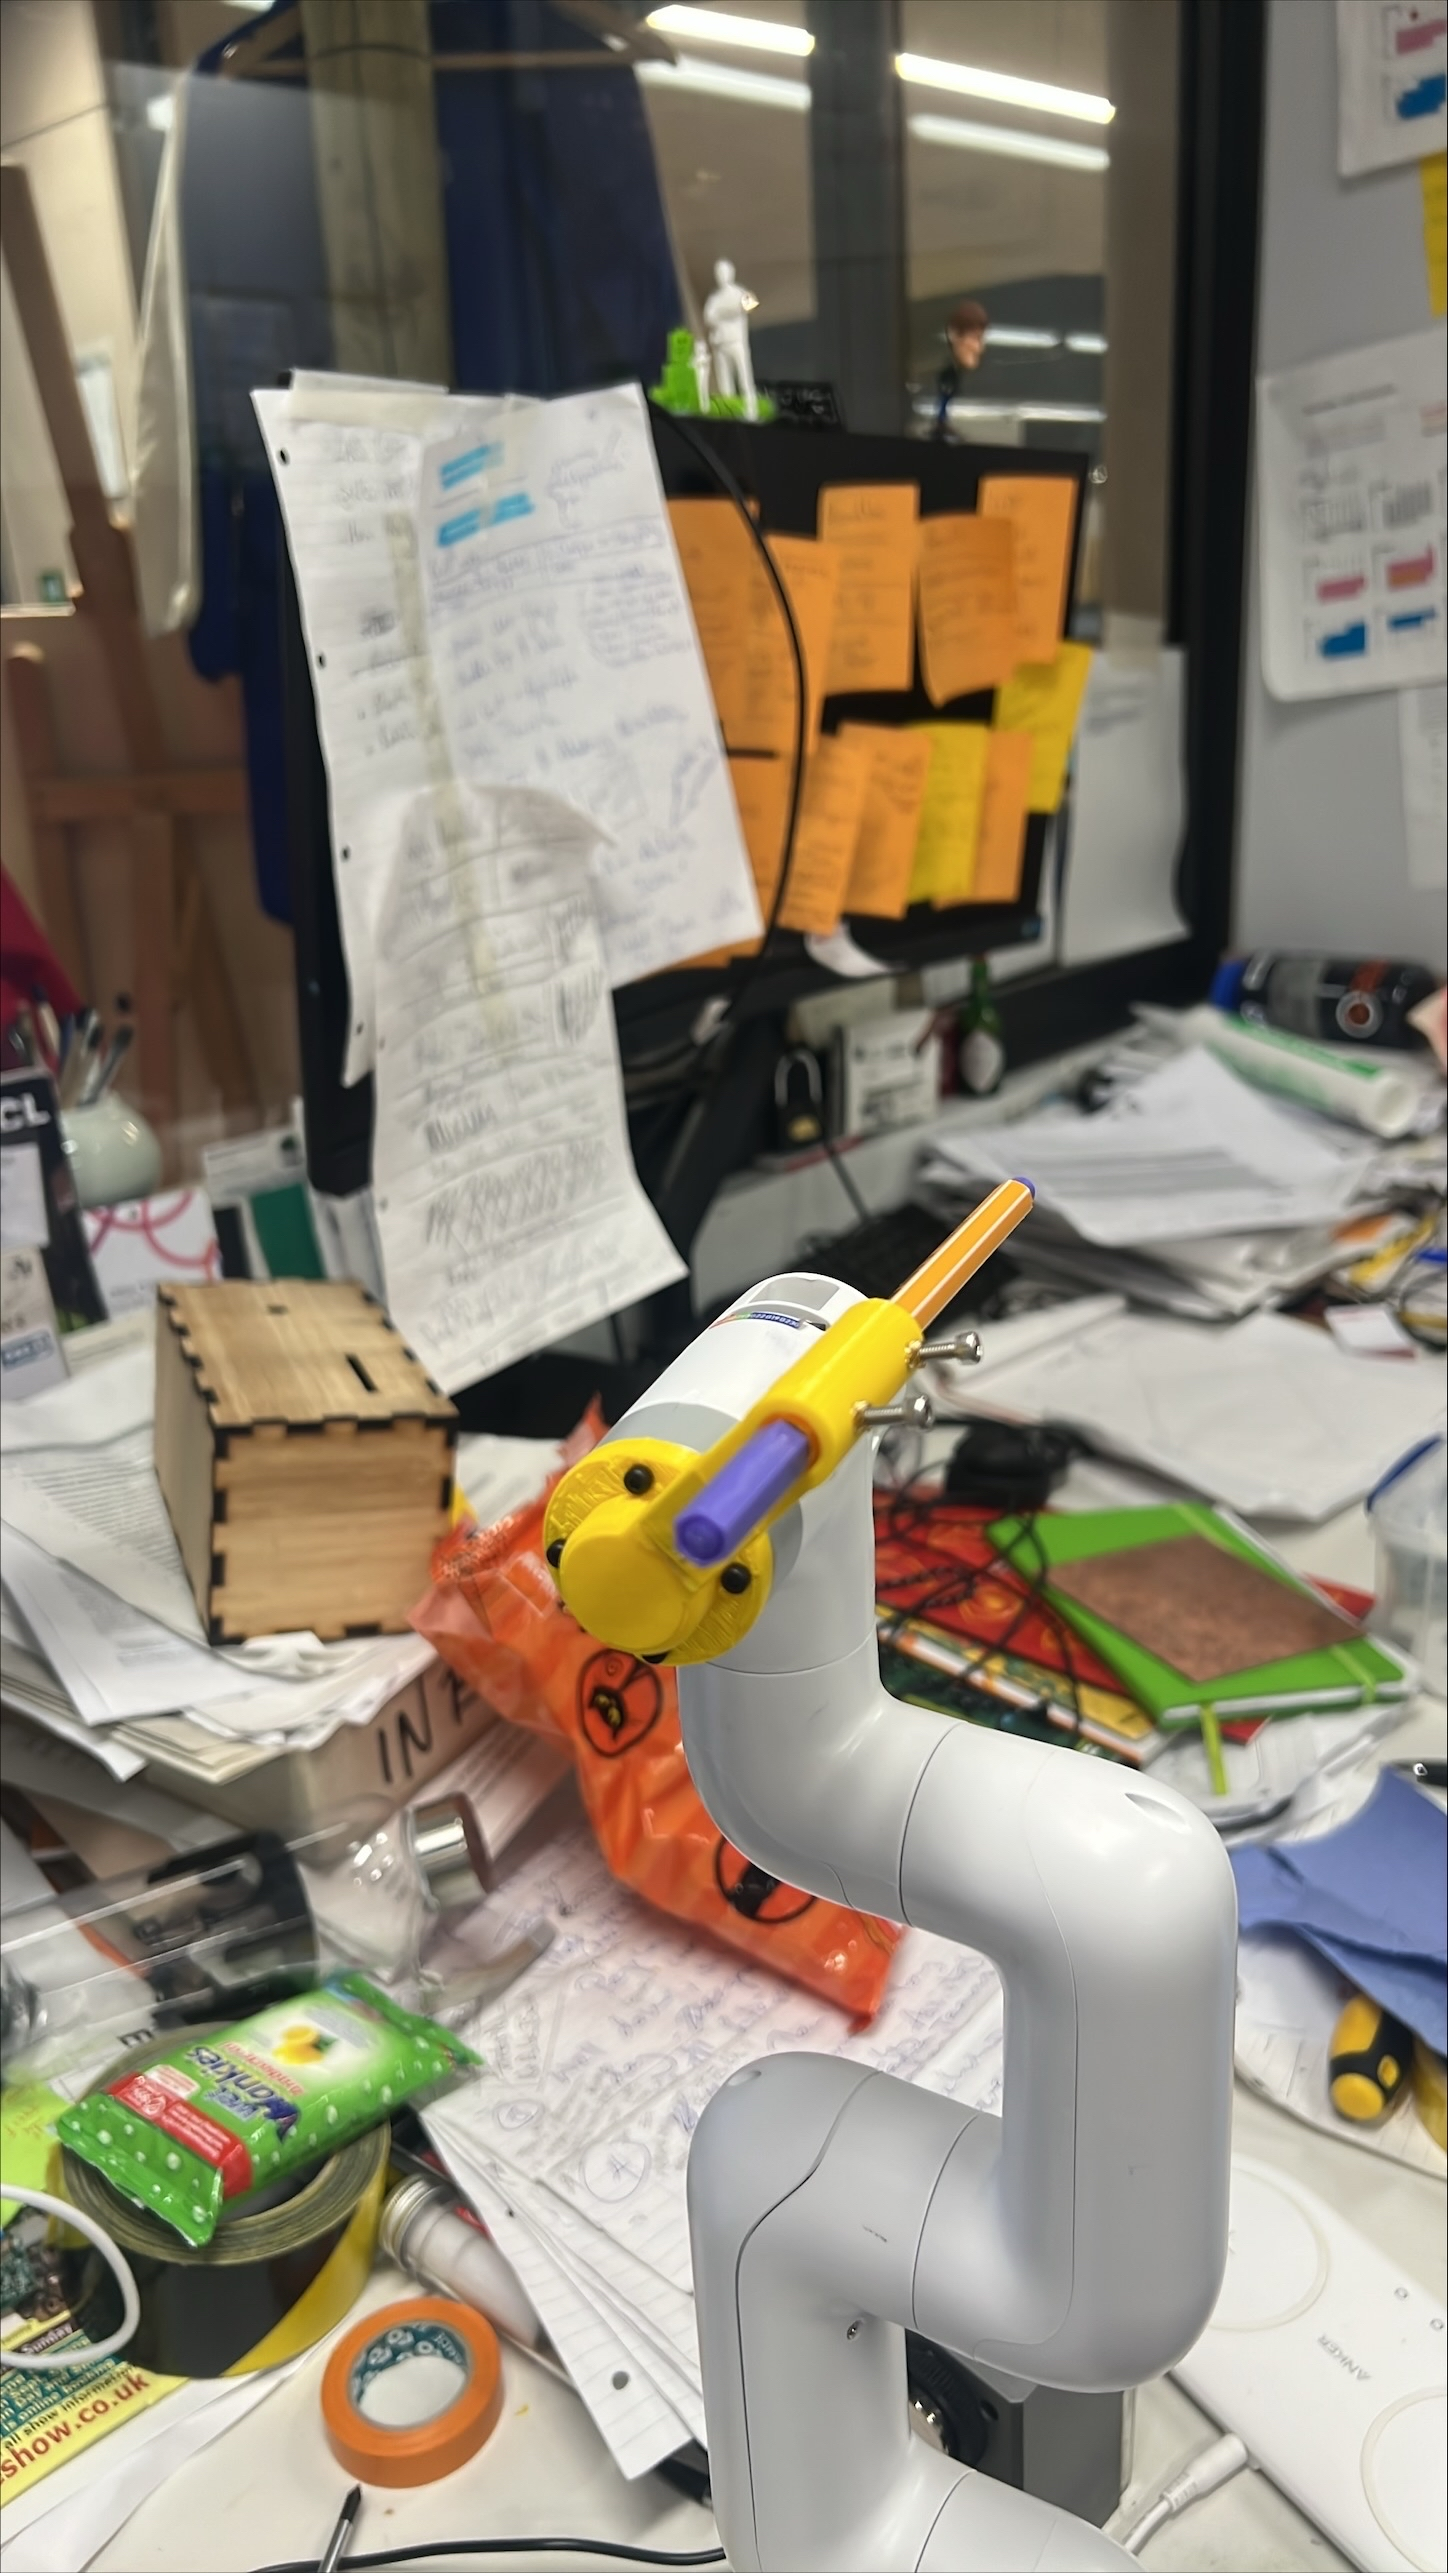
\includegraphics[width=8cm]{figures/marker_mount.jpeg}
\centering
\caption{Mounting system as designed and fabricated by Alex Charitonidis is shown for the marker to attach to the MyCobot Robot Arm.}
\label{fig:pen_mount}
\end{figure}

\textcolor{red}{Model the base of the robot and the pen tip in the DH parameters. Include a picture of the new kinematic diagram and also modify the DH parameters included in the ros\_arm\_controller package in ros\_arm\_controller/constants.py and include the modified parameters. Hint: it may be helpful to use two frames for the pen, one to the middle of the pen and one to the tip. The tip is what we care about. It may also help to match Pybullet's coordinate frame for the tip so as to more easily compare IK solutions later (press W and then J in pybullet to see frames).}

\textcolor{blue}{Answer: }


\subsection{Question 2--Coding up DH Params}

Complete the function standard\_dh in ros\_arm\_controller/kinematics.py to calculate a transform matrix from a set of parameters and the function get\_transform\_last\_frame in the same file to chain these to get the transform to the tip of the pen.

\textcolor{red}{ What is the task space vector that ensues from a configuration $q = \begin{bmatrix} 0.0& \frac{\pi}{2}& \frac{\pi}{2}& 0.0& 0.0& 0.0 \end{bmatrix}^T$? }

\textcolor{blue}{Answer: }


\clearpage
\section{Inverse Kinematics}

Another fundamental problem in robotics is going from a desired XYZ position of the robot's end effector, like a gripper trying to pick up a box at a known location, to joint angles to achieve the goal. This is inverse kinematics and this section will explore this problem.

\subsection{Question 1--Inverse Kinematics}
Gradient ascent is a popular method to iteratively calculate a solution to inverse kinematics. One method is detailed in \cite{wolovich1984computational}. 

We will implement a numerical solution that comes from minimizing a squared error function between current pose and desired pose and results in an iterative method based on gradient ascent. Equation \eqref{eq:ik} details this, where we set $r \in \mathcal{R}^6$ to be the task vector which includes position in x, y, and z (in meters), and orientation around the x, y, and z axis (using Euler angles in radians and RPY convention), the configuration space $q \in \mathcal{R}^6$ represents joint angles of the robot arm, the jacobian matrix of the forward kinematics map, calculated via Jax which is an autogradient framework, $J_r(q) = \frac{\partial f_r(q)}{\partial q}$, and the forward kinematics map is a function to go from joint angles to task space $f_r(q^k)$, $\alpha$ is a hyperparameter that represents step size where too large values may cause the iteration to miss the minimum and too low values may cause slow convergence, and $K>0$ is a gains matrix used to accelerate convergence (and accomodate varying units on the task vector $r$ between meters and radians). When error between the desired task vector and the task vector from forward kinematics is under some tolerance, we exit iterating. There are some pitfalls to this method, including: the importance of an initial guess where different initial guesses will ensue in different solutions to the IK; optimal step size can be difficult to tune; and understanding closeness to singularities. That said, this is one of the more approachable IK methods to implement.

\begin{align}
q^{k+1} =& q^k + \alpha J_r^T (q^k) K \left[ r_d - f_r(q^k) \right] \label{eq:ik}
\end{align}

Populate the function get\_ik to do so in the file ros\_arm\_controller/kinematics.py, assuming that orientation is not provided and it is only position.


\textcolor{red}{ What is a solution to the task vector $r=\begin{bmatrix} 0.2& 0.15& 0.005\end{bmatrix}^T$ and how many iterations does it take from an initial configuration of $q = \begin{bmatrix} 0.0& 0.0& 0.0& 0.0& 0.0& 0.0 \end{bmatrix}^T$?}

\textcolor{blue}{Answer: }


In the trajectory.py file within ros\_arm\_controller package there is a parameter use\_pybullet\_for\_ik. Set this to false to use your method. Then run the controller along with the simulator to follow a line (commands in README), without orientation. A pybullet class with an IK solver is included to compare your work.

\textcolor{red}{Include a screenshot of the robot following a line, without orientation.}

\textcolor{blue}{Answer: }

When performing gradient ascent a variety of schemes may be used including jacobian tranpose, jacobian inverse, and jacobian pseudoinverse.

\textcolor{red}{What are some of the tradeoffs between jacobian tranpose, jacobian inverse, and jacobian pseudoinverse approaches to solving IK.}

\textcolor{blue}{Answer: }

Include orientation in the IK by leveraging a gains matrix that is positive semidefinite to scale position error and orientation error.

Note the tuning parameters including number of iterations, gradient step size, and gains matrix.

\textcolor{red}{What are the tuning parameters you settle on to achieve a line with orientation including number of iterations, gradient step size, and gains matrix.}

\textcolor{blue}{Answer: }

\clearpage
\section{Trajectory Following}

With the given pieces of forward kinematics and inverse kinematics, we can now design a trajectory as a series of poses (position and orientation or just position) in 3D space.

\subsection{Question 1--Designing a Trajectory}

The trajectory.py file inside of the ros\_arm\_controller package provides joint interpolation and line trajectory segment functionality. Look at the inputs to the interpolate\_joint\_angles function and the draw\_line function. 

\textcolor{red}{Compare the interpolate\_joint\_angles function and the draw\_line function. Which is computationally more expensive? Which would you use for longer moves where the position of the end effector isn't crucial. Which would you use for shorter moves where the position of the end effector is critical?}

\textcolor{blue}{Answer: }

Decide on a goal shape like a first letter from your name and populate the traj\_key\_segments member of the TrajectoryPlanner class using both joint interpolation and line trajectory segments. Hint: small steps between waypoints when solving IK are useful and faster to solve. Care must be taken to be inside of the workspace of the robot and to have a feasible pose (position and orientation). It is recommended to start slow with easier short trajectories and build from them.

Run your trajectory, tuning parameters for the IK solve.

\textcolor{red}{Describe your planned trajectory including its shape, starting point and ending point. Include the graphs generated by robo\_controller.py of the planned and actual trajectories. How long did the solve take? How much error do you have in the actual trajectory?}

\textcolor{blue}{Answer: }


\clearpage
\section{Real Robot}

We now will mimick this work on the Mycobot 280 Raspberry Pi. Follow the instructions in the README to run your work on the real robot. Tuning of parameters may be needed.

\textcolor{red}{Include a picture of the real robot following your trajectory as well as the actual trajectory and planned trajectory generated by robo\_controller.py. How much error does the real robot have? How does this compare to the simualated robot, and what are some of the changes needed to get this running on the real robot?}

\textcolor{blue}{Answer: }

By running the same trajectory multiple times, you can get an idea of repeatability of the robot and how closely it mimicks prior actions.

\textcolor{red}{ How does the real robot perform on repeatability, in comparison to the simulated robot?}

\textcolor{blue}{Answer: }

\clearpage
\section{Moveit 2}

In industry, while it is critical to understand forward and inverse kinematics (and implementing algorithms is a great way to build understanding), it is rare for practioners to implement forward kinematic or inverse kinematics themselves. This is because it takes time that practioners may prefer to spend on their value-add--most businesses do not try to add value by solving FK and IK themselves, as an example they may sell a pool-cleaning robot and may prefer to focus on making the robot resistant to water or path-planning in a pool. Additionally, re-coding the wheel risks introducing errors. Practioners most often use a library that implements these kinematic algorithms, with some exceptions in special circumstances. Figure \ref{moveit2_cobot} shows Moveit2, a popular library for working with robot arms.

\begin{figure}[h]
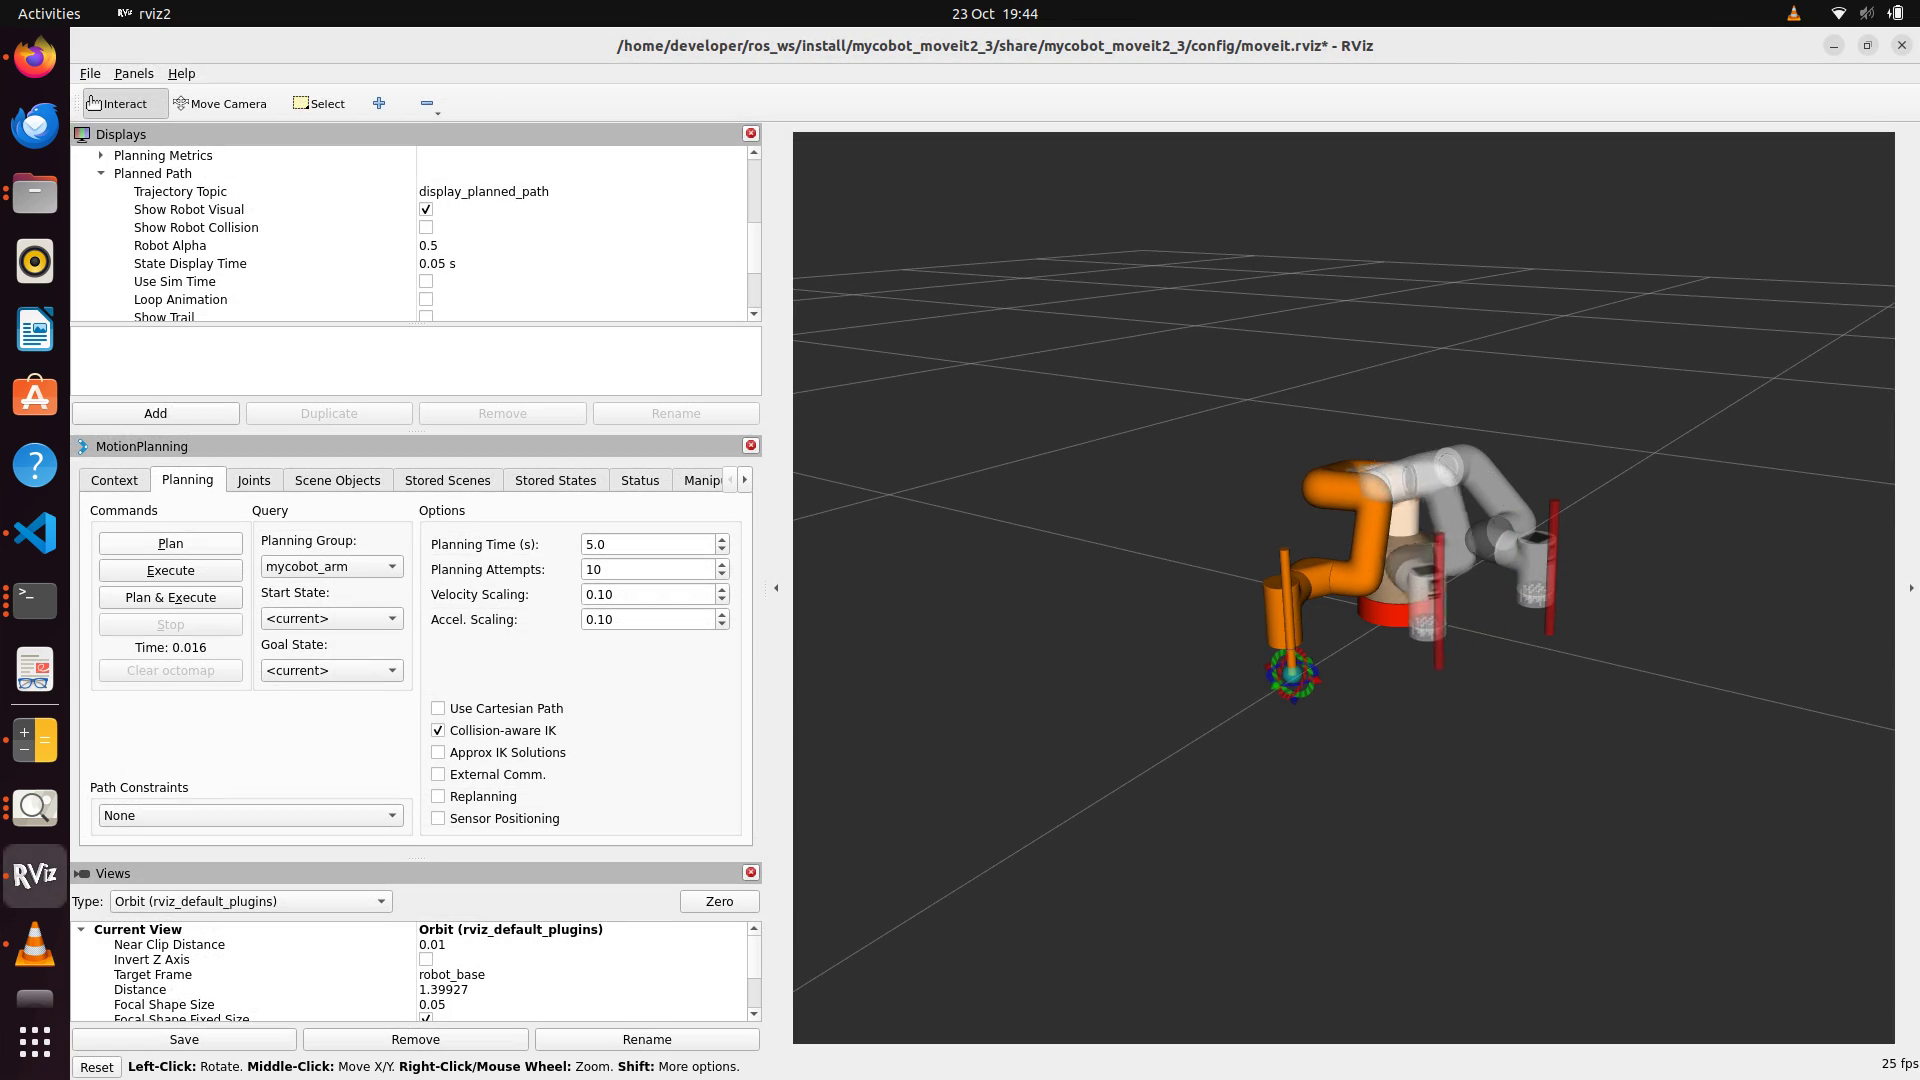
\includegraphics[width=8cm]{figures/moveit2_cobot.png}
\centering
\caption{Screenshot of RVIZ2 while using Moveit 2 to control the mycobot arm, with no self-written code.}
\label{moveit2_cobot}
\end{figure}

Follow the instructions in the README to get the arm moving. Experiment with trajectories using collision aware IK and comparing to IK without collision awareness.


\textcolor{red}{How is the experience using moveit2? If you had to do another trajectory for a different letter in the English alphabet, with your current knowledge of moveit2, how much time and effort would it take to do this using moveit2 in comparison to using the code you've written in the above sections? What about once you have worked with moveit2 for some time?}

\textcolor{blue}{Answer: }

\clearpage

\bibliographystyle{IEEEtran}
\bibliography{refs}

\end{document}
